\documentclass[10pt]{article}
\pdfminorversion=4

\usepackage{amssymb}
\usepackage{pslatex,palatino,avant,graphicx,color}
\usepackage{colortbl}
\usepackage{fullpage}
\usepackage{mathtools}
\usepackage{natbib}
\usepackage{amsmath}
\usepackage{caption}
%\usepackage{subfigure}
\usepackage{subcaption}
\usepackage{bm}
\usepackage{wrapfig}
\usepackage{enumerate}
\usepackage{rotating}
\usepackage{multirow}
\usepackage{tabularx}
\usepackage{tikz}
\usepackage{pgfplots}
\usepackage{bbm}
\usepackage[titles,subfigure]{tocloft} % Alter the style of the Table of Contents

%\pdfminorversion=4
% NOTE: To produce blinded version, replace "0" with "1" below.
\newcommand{\blind}{0}

% DON'T change margins - should be 1 inch all around.
\addtolength{\oddsidemargin}{-.5in}%
\addtolength{\evensidemargin}{-.5in}%
\addtolength{\textwidth}{1in}%
\addtolength{\textheight}{1.3in}%
\addtolength{\topmargin}{-.8in}%


\renewcommand{\cftsecfont}{\rmfamily\mdseries\upshape}
\renewcommand{\cftsecpagefont}{\rmfamily\mdseries\upshape} % No bold!

\newcommand{\indicator}[1]{\mathbbm{1}\left( #1 \right) }
\newcommand{\hb}{\hat{b}}
\newcommand{\ha}{\hat{a}}
\newcommand{\htheta}{\hat{\theta}}
\newcommand{\halpha}{\hat{\alpha}}
\newcommand{\hmu}{\hat{\mu}}
\newcommand{\hsigma}{\hat{\sigma}}
\newcommand{\hphi}{\hat{\phi}}
\newcommand{\htau}{\hat{\tau}}
\newcommand{\heta}{\hat{\eta}}
\newcommand{\E}[1]{\mbox{E}\left[#1\right]}
\newcommand{\Var}[1]{\mbox{Var}\left[#1\right]}
\newcommand{\Indicator}[1]{\mathbbm{1}_{ \left( #1 \right) } }
\newcommand{\dNormal}[3]{ N\left( #1 \left| #2, #3 \right. \right) }
\newcommand{\Beta}[2]{\mbox{Beta}\left( #1, #2 \right)}
\newcommand{\alphaphi}{\alpha_{\hphi}}
\newcommand{\betaphi}{\beta_{\hphi}}
\newcommand{\expo}[1]{ \exp\left\{ #1 \right\}}
\newcommand{\tauSquareDelta}{\htau^2
  \left(\frac{1-\expo{-2\htheta\Delta}}{2\htheta} \right)}
\newcommand{\mumu}{\mu_{\hmu}}
\newcommand{\sigmamu}{\sigma^2_{\hmu}}
\newcommand{\sigmamuexpr}{\log\left( \frac{\VarX}{\EX^2} + 1 \right)}
\newcommand{\mumuexpr}{\log(\EX) -  \log\left( \frac{\VarX}{\EX^2} + 1 \right) /2 }

\newcommand{\EX}{\mbox{E}\left[ X \right] }
\newcommand{\VarX}{\mbox{Var}\left[ X \right] }
\newcommand{\mueta}{\mu_{\heta} }
\newcommand{\sigmaeta}{\sigma^2_{\heta}}
\newcommand{\sigmaetaexpr}{ \log\left( \frac{\VarX}{\EX^2} + 1 \right) }
\newcommand{\muetaexpr}{ \log(\EX) -  \sigmaetaexpr /2 }

\newcommand{\mualpha}{\mu_{\halpha} }
\newcommand{\sigmaalpha}{\sigma^2_{\halpha}}
\newcommand{\sigmaalphaexpr}{ \log\left( \frac{\VarX}{\EX^2} + 1 \right) }
\newcommand{\mualphaexpr}{ \log(\EX) -  \sigmaalphaexpr /2 }

\newcommand{\mutauexpr}{ \frac{2}{T} \EX }
\newcommand{\sigmatauexpr}{ \frac{4}{T^2} \Var{X}}

\newcommand{\alphatau}{\alpha_{\htau^2}}
\newcommand{\betatau}{\beta_{\htau^2}}

\newcommand{\Gam}[2]{\mbox{Gamma}\left( #1, #2 \right) }
\newcommand{\InvGam}[2]{\mbox{Inv-Gamma}\left( #1, #2 \right) }

%%% END Article customizations

%%% The "real" document content comes below...

% \newbox{\LegendeA}
% \savebox{\LegendeA}{
%    (\begin{pspicture}(0,0)(0.6,0)
%    \psline[linewidth=0.04,linecolor=red](0,0.1)(0.6,0.1)
%    \end{pspicture})}
% \newbox{\LegendeB}
%    \savebox{\LegendeB}{
%    (\begin{pspicture}(0,0)(0.6,0)
%    \psline[linestyle=dashed,dash=1pt 2pt,linewidth=0.04,linecolor=blue](0,0.1)(0.6,0.1)
%    \end{pspicture})}

\title{Solution to a Non-Seperable Diffusion Equation on a Regular Domain}
\author{Georgi Dinolov, Abel Rodriguez, Hongyun Wang}
\date{} % Activate to display a given date or no date (if empty),
         % otherwise the current date is printed 

\begin{document}
\def\spacingset#1{\renewcommand{\baselinestretch}%
{#1}\small\normalsize} \spacingset{1}

\bigskip

\abstract{}

\vspace{1cm}
\noindent
{\it Keywords:} Diffusion equation, regular bounded domain

\spacingset{1.00} % DON'T change the spacing! was set to 1.45
\section{Motivation}\label{se:motivation}

\section{Solution on $\Omega \subset \mathbb{R}$}

In this Section we will demonstrate the method outlined in Section
\ref{se:motivation} where the solution is defined on a bounded
interval on $\mathbb{R}$. In this case, we have the true solution to
the diffusion equation. We will compare the asymptotic
expansion to the true solutio.

The PDE we will solve is the following BC/IC problem
\begin{align}
  \frac{\partial}{\partial t} q(x,t) &= \frac{1}{2}\sigma^2 \frac{\partial^2}{\partial x^2} q(x,t), \label{eq:pde} \\
  q(x,0) &= \delta_{x_0}(x), \label{eq:ic} \\
  q(a,t) &= q(b,t) = 0. & (\mbox{i.e. } \Omega = [a,b]) \label{eq:bc}
\end{align}
\textbf{Without loss of generality we will assume}
\begin{align*}
  a &=0, & b &= 1.
\end{align*}

Problem (\ref{eq:pde}) - (\ref{eq:bc}) can be solved in a variety of
ways. We will use the method of images, which repeatedly reflects the
fundamental solution
\[
  q_{fundamental}(x,t) = \frac{1}{\sqrt{2\pi \sigma^2 t}} \exp\left\{ -\frac{1}{2\sigma^2t} (x-x_0)^2 \right\}
\]
about the boundary points $a$ and $b$. The steps for the full
solutions are as follows:

\begin{enumerate}[Step 1:]
\item Select a kernel $f(x|t)$ for the basis expansion,
\item Perform Gram-Schmidt orthogonalization on the polynomials basis,
\item Compute the weight for each basis element,
\item Profit.
\end{enumerate}

\subsection{A suitable kernel for the basis elements}
As noted in the motivating Section \ref{se:motivation}, the kernel we
will use must be in $C^{\infty}(a,b)$, and it must obey the boundary
conditions. Moreover, the basis kernel must be chosen such that
\begin{enumerate}[i)]
\item derivatives $f'(x)$ can be computed easily, 
\item integrals $\int_{\Omega} x^m f(x|t)^2\, dx$ can be computed easily
\end{enumerate}
Consideration i) suggests that $f(x|t)$ should be of polynomial
form. Consideration ii) suggests that $f(x|t)$ should be a known pdf
over $[a,b]$, taking on zero at $a$ and $b$.  Given these
requirements, the Beta distribution comes to mind:
\[
  f(x|t, \alpha, \beta) = \frac{1}{B(\alpha,\beta)} x^{\alpha-1}(1-x)^{\beta-1},
\]
where $B(\alpha,\beta)$ is the beta function. Our choice for $\alpha$
and $\beta$ is not very restricted. However, we will outline a few
heuristics by which we can choose these parameters. Note that there
may exist and optimal choise for $(\alpha, \beta)$ in terms of the
accuracy of the asymptotic expansion with respect to the true solution
$q(x,t)$. However, we will not prove anything in this vein here.

\textbf{First}, as long as
\begin{align}
  \alpha, \beta > 1, \label{eq:lower-bound}
\end{align}
the mode for the distribution is guaranteed to
exist, so that the boundary conditions are met.

Aside from $\alpha > 1$ and $\beta > 1$, we can pick any
$(\alpha,\beta)$ pair for our kernel. However, given that $f(x|t)$ can
be thought of as implicitly dependent upon $t$, and that the variance
of the fundamental solution is $\sigma^2t$, a first, reasonable guess
for $(\alpha,\beta)$ can be given by the solution to the equation:
\begin{align}
  \Var{X} &:= \frac{\alpha \beta}{(\alpha+\beta)^2(\alpha+\beta+1)} = \sigma^2t, \label{eq:var-restriction}\\
  p(X \in dx) &= f(x|t, \alpha, \beta). \nonumber
\end{align}

By the same logic, noting the mean for the fundamental solution, we can require
\begin{align}
  \E{X} &:= \frac{\alpha}{\alpha+\beta} = x_0, \label{eq:mean-restriction}\\
  p(X \in dx) &= f(x|t, \alpha, \beta). \nonumber
\end{align}

Finally, we may require that $\alpha, \beta \in \mathbb{Z}$, since
this will guarantee that
\[
  \frac{\partial^k}{\partial x^k} f(x|t,\alpha,\beta) = 0
\]
for large enough $k$. [georgid: This may not prove important, but I
will keep it here anyway]

Thus, to set $\alpha$ and $\beta$, we simultaneously solve
(\ref{eq:var-restriction}) and (\ref{eq:mean-restriction}), then round
$\alpha$ and $\beta$ to the closest integer greater than or equal to
2. Since $\alpha$ and $\beta$ are dependent upon $t$, we will keep $t$
in our notation for $f$, albeit implicitly. In other words, once we
choose $\alpha$ and $\beta$, we will not be able to take derivatives
of $f$ with respect to $t$. We will denote the kernel as
$f(x| \alpha, \beta ; t)$.

\subsection{Gram-Schmidt orthogonalization on the polynomials basis}
The family of (polynomial) functions
$\left\{ x^m f(x| \alpha, \beta; t) \right\}_{m=0}^\infty$ spans the
space of $L^2([a,b])$ functions. We generate the basis elements
$\left\{ u_m(x|\alpha,\beta;t) \right\}_{m=0}^\infty$ by setting
\begin{align}
  v_0(x| \alpha, \beta; t) &= f(x| \alpha, \beta; t), \nonumber \\
  u_0(x| \alpha, \beta; t) &= \frac{f(x| \alpha, \beta; t)}{\|f(x|\alpha, \beta; t\|}, \label{eq:u0} \\
  \|f(x|\alpha,\beta;t) \| &\equiv \left( \int_{\Omega} f(x|\alpha,\beta;t)^2 dx \right)^{1/2}. \label{eq:norm}
\end{align}
The integral in (\ref{eq:norm}) is easy to compute because of the form
we have chosen for the kernel $f:$
\begin{align*}
  \int_{\Omega} f(x|\alpha,\beta;t)^2 dx  &= \int_{\Omega} \left( \frac{1}{B(\alpha,\beta)} x^{\alpha-1}(1-x)^{\beta-1} \right)^{2} dx, \\
                                          &= \int_{\Omega} \frac{1}{B(\alpha,\beta)^2} x^{(2\alpha-1)-1}(1-x)^{(2\beta-1)-1} dx, \\
                                          &= \frac{B(2\alpha-1, 2\beta-1)}{B(\alpha,\beta)^2}, \\
  \left( \int_{\Omega} f(x|\alpha,\beta;t)^2 dx \right)^{1/2} &= \sqrt{\frac{B(2\alpha-1, 2\beta-1)}{B(\alpha,\beta)^2}}.
\end{align*}
Next, for $u_1(x;\alpha,\beta;t)$,
\begin{align}
  v_1(x| \alpha, \beta; t) &= x f(x|\alpha,\beta;t) - \left<x f(x|\alpha,\beta;t) | u_0(x|\alpha,\beta;t) \right> u_0(x|\alpha,\beta;t) \\
  &= \left(x - \frac{\left<x f(x|\alpha,\beta;t) | u_0(x|\alpha,\beta;t) \right>}{\| f(x|\alpha,\beta;t) \|} \right) f(x|\alpha,\beta;t) \\
  \left<x f(x|\alpha,\beta;t) | u_0(x|\alpha,\beta;t) \right> &= \int_\Omega \frac{x f(x|\alpha,\beta;t)^2}{\| f(x|\alpha,\beta;t) \|} = \frac{1}{\| f(x|\alpha,\beta;t) \|} \int_\Omega \frac{1}{B(\alpha,\beta)^2} x^{2\alpha-1}(1-x)^{(2\beta-1)-1} dx  \\
  u_1(x|\alpha,\beta;t) &= \frac{v_1(x|\alpha,\beta;t)}{\|v_1(x|\alpha,\beta;t)\|} \\
  \|v_1(x|\alpha,\beta;t)\| &= \int_\Omega \left(x - \frac{\left<x f(x|\alpha,\beta;t) | u_0(x|\alpha,\beta;t) \right>}{\| f(x|\alpha,\beta;t) \|} \right)^2 f(x|\alpha,\beta;t)^2 dx \\
  u_1(x|\alpha,\beta;t) &= \frac{v_1(x|\alpha,\beta;t)}{\|v_1(x|\alpha,\beta;t)\|} = p_1(x) f(x|\alpha,\beta;t), 
\end{align}
where $p_1(x)$ is a first-order polynomial. In general,
\begin{align*}
  v_{m}(x|\alpha,\beta;t) &= x^m f(x|\alpha,\beta;t) - \sum_{m'=0}^{m-1} \left< x^m f(x|\alpha,\beta;t) | u_{m'}(x|\alpha,\beta;t) \right>u_{m'}(x|\alpha,\beta;t) \\
  u_{m}(x|\alpha,\beta;t) &=  \frac{v_{m}(x|\alpha,\beta;t)}{\| v_{m}(x|\alpha,\beta;t) \|}  \equiv p_m(x|\alpha,\beta;t) f(x|\alpha,\beta;t)
\end{align*}
In finding the basis, we will have to perform two main types
calcluations:
\begin{enumerate}[1)]
\item polynomial multiplication: $p_m(x|\alpha,\beta;t)p_n(x|\alpha,\beta;t)$
\item integration of the form: $\int_\Omega x^m f(x|\alpha,\beta;t)^2 dx$
\end{enumerate}
In \texttt{R}, the package \texttt{mpoly} will be used to handle
1). Calculation 2) can be performed relatively easily due to the form
of $f(x|\alpha,\beta;t)$, as show in (\ref{eq:intpoly}).

\begin{align}
  \int_\Omega x^m f(x|\alpha,\beta;t)^2 dx &= \int_\Omega x^m \frac{1}{B(\alpha,\beta)^2} x^{2\alpha-2}(1-x)^{2\beta-2} dx = \frac{1}{B(\alpha,\beta)^2} \int_\Omega x^{2\alpha+m-2}(1-x)^{2\beta-2} dx = \frac{B(2\alpha+m-1, 2\beta-1)}{B(\alpha,\beta)^2} \label{eq:intpoly}
\end{align}

\subsection{Computing the Weights of the Basis Elements}
Given the set of orthonormal functions
$\{u_m(x|\alpha,\beta;t)\}_{m=0}^\infty$ spanning $L^2([a,b])$, and
assuming that $q(x,t) \in L^2([a,b])$, we can write down
\begin{align}
   q(x,t) &= \sum_{m=0}^\infty c_m u_m(x|\alpha,\beta;t), \\
  \mbox{with  } c_m &= \int_\Omega q(x,t) u_m(x|\alpha,\beta;t) dx. \label{eq:coef}
\end{align}
Since each $u_m$ is the product of two polynomials,
$u_m(x|\alpha,\beta;t) \in C^{\infty}([a,b])$ and is
square-integrable. Therefore, we can write
\begin{equation}
  \int_\Omega \frac{\partial^k \delta_{x_0}(x)}{\partial x^2}
  u_m(x|\alpha,\beta;t) dx = (-1)^{k} \int_\Omega \delta_{x_0}(x)
  \frac{\partial^k u_m(x|\alpha,\beta;t)}{\partial x^k} dx = (-1)^k
  \left. \frac{\partial^k u_m(x|\alpha,\beta;t)}{\partial x^k}
  \right|_{x=x_0} \label{eq:delta-deriv}
\end{equation}
Equipped with (\ref{eq:delta-deriv}) and that
$q(x,0) = \delta_{x_0}(x)$, we can compute the integrals in
(\ref{eq:coef}) by using the Taylor expansion of $q(x,t)$ about $t=0$:
\begin{align*}
  c_m(t; \alpha,\beta,x_0) = \int_\Omega q(x,t) u_m(x|\alpha,\beta;t) dx
  &= \int_\Omega \left[\underbrace{q(x,0)}_{\delta_{x_0}(x)} +
    \sum_{k=1}^\infty \frac{t^k}{k!} \left. \frac{\partial^k q(x,t)}{\partial t^k} \right|_{t=0} \right] u_m(x|\alpha,\beta;t) dx \\
                                                                         &= \int_\Omega \delta_{x_0}(x) u_m(x|\alpha,\beta;t) dx + \sum_{k=1}^\infty \frac{t^k}{k!} \int_\Omega \left. \frac{\partial^k q(x,t)}{\partial t^k} \right|_{t=0} u_m(x|\alpha,\beta;t) dx \\
                                                                         &= \int_\Omega \delta_{x_0}(x) u_m(x|\alpha,\beta;t) dx + \sum_{k=1}^\infty \frac{t^k}{k!} \int_\Omega \left(\frac{1}{2}\sigma^2\right)^{k} \frac{\partial^{2k} \delta_{x_0}(x)}{\partial x^{2k}} u_m(x|\alpha,\beta;t) dx \\
                                                                         &= u_m(x_0|\alpha,\beta;t) + \sum_{k=1}^\infty \frac{t^k}{k!} (-1)^{2k} \left(\frac{1}{2}\sigma^2\right)^{k} \int_\Omega \delta_{x_0}(x) \frac{\partial^{2k} u_m(x|\alpha,\beta;t)}{\partial x^{2k}} dx \\
                                              &= u_m(x_0|\alpha,\beta;t) + \sum_{k=1}^\infty \frac{t^k}{k!} (-1)^{2k} \left(\frac{1}{2}\sigma^2\right)^{k}\frac{\partial^{2k} u_m(x_0|\alpha,\beta;t)}{\partial x^{2k}} \\
                                                                         &= u_m(x_0|\alpha,\beta;t) + \sum_{k=1}^\infty \frac{t^k}{k!} \left(\frac{1}{2}\sigma^2\right)^{k} \frac{\partial^{2k} u_m(x_0|\alpha,\beta;t)}{\partial x^{2k}}.
\end{align*}

Note that
\begin{align*}
  u_m^{(k)}(x|\alpha,\beta;t) &= \sum_{j=0}^k \left(\begin{array}{c}
                                                      k \\
                                                      j
                                                      \end{array} \right)
  p^{(j)}_m(x|\alpha,\beta;t) f^{(k-j)}(x|\alpha,\beta;t) \\
  f'(x|\alpha,\beta;t) &= \frac{1}{B(\alpha,\beta)}
                         \left[(\alpha-1)x^{\alpha-2}(1-x)^{\beta-1}
                         + (\beta-1)x^{\alpha-1}(1-x)^{\beta-2} \right] \\
                         &= \frac{1}{B(\alpha,\beta)}
                         \left[(\alpha-1)B(\alpha-1,\beta) f(x|\alpha-1,\beta;t)
                           + (\beta-1)B(\alpha,\beta-1)
                           f(x|\alpha,\beta-1;t) \right] \\
\end{align*}

The $k^{th}$ order derivative of the polynomial $p_m(x|\alpha,\beta;t)$ can be
computed on the fly with \texttt{mpoly}. The recursive definition of 

\section{Another Kernel Choice}
Another suitable kernel choise the bump function
\begin{align}
  f(x) &= \left\{ \begin{array}{cc}
                    \exp\left\{ -\frac{1}{1-x^2} \right\}, &\mbox{if } |x|<1 \\
                    0, &\mbox{otherwise}
                  \end{array} \right.
\end{align}
In thise case, $f \in C^\infty(-1,1).$ As outlined perviously, we need to compute
\begin{align*}
  f^{(k)}(x), &  \int_{-1}^1 x^m f(x)^2 \,dx  &
\end{align*}
For the first calculation, note that
\begin{align*}
  f'(x) &= f(x)(1-x^2)^{-2}(-2x) \equiv f(x)P_{1,0}(x)^{-1} P_{1,1}(x)
\end{align*}
Assuming that
\[
  f^{(k)}(x) = f(x)P_{k,0}(x)^{-1}P_{k,1}(x),
\]
we have that
\begin{align*}
  f^{(k+1)}(x) &= f'(x)P_{k,0}(x)^{-1}P_{k,1}(x) \\
               &&+ f(x)\left[ -P_{k,0}(x)^{-2}P_{k,0}'(x)P_{k,1}(x)
                 + P_{k,0}(x)^{-1}P_{k,1}'(x) \right] \\
               &= \left( f(x)P_{1,0}(x)^{-1} P_{1,1}(x) \right)P_{k,0}(x)^{-1}P_{k,1}(x) \\
               &&+ f(x)P_{k,0}(x)^{-2}\left[ -P_{k,0}'(x)P_{k,1}(x)
                  + P_{k,0}(x)P_{k,1}'(x) \right] \\
               &= f(x) \left(P_{k,0}(x)P_{1,0}(x)\right)^{-1} P_{1,1}(x) P_{k,1}(x)\\
                 &&+f(x)P_{k,0}(x)^{-2}\left[ -P_{k,0}'(x)P_{k,1}(x)
                 + P_{k,0}(x)P_{k,1}'(x) \right]
\end{align*}

\[
  f^{(k+1)}(x) =
  f(x)\left[P_{k,0}(x)P_{1,0}(x)P_{k,0}(x)^2\right]^{-1} \left(
    P_{1,1}(x) P_{k,1}(x)P_{k,0}(x)^2 + P_{k,0}(x)P_{1,0}(x)\left[
      -P_{k,0}'(x)P_{k,1}(x) + P_{k,0}(x)P_{k,1}'(x) \right] \right)
\]

\[ \boxed{ P_{k+1,0} = P_{k,0}(x)P_{1,0}(x)P_{k,0}(x)^2 } \]
\[ \boxed{ P_{k+1,1} = P_{1,1}(x) P_{k,1}(x)P_{k,0}(x)^2 +
    P_{k,0}(x)P_{1,0}(x)\left[ -P_{k,0}'(x)P_{k,1}(x) +
      P_{k,0}(x)P_{k,1}'(x) \right] } \]

\section{Mesh-Free Finite Element Method}
Here we take a similar approach, where we seek the \textit{weak
  solution} of the PDE (\ref{eq:pde}) - (\ref{eq:bc}). A weak solution
is any function $q_{weak}(x,t)$ where, for any
$\phi(x) \in C^{\infty}_0(\Omega)$,
\begin{align}
  \displaystyle \int_\Omega \partial_t q_{weak}(x,t) \phi(x)\, dx -
  \frac{1}{2}\sigma^2 \displaystyle \int_\Omega \partial^2_x q_{weak}(x,t) \phi(x)\,dx = 0. \label{eq:weak-sol}
\end{align}
We can relax the definition of a weak solution in the following
way. Consider a countable family of functions, or elements,
$\left\{\psi_k(x)\right\}_{k=1}^\infty$ dense in the space of all
$L_2(\Omega)$ functions. It can be shown that a function is a weak
solution to the problem if (\ref{eq:weak-sol}) holds for each
$\psi_k(x)$. In other words,
\begin{align}
  \displaystyle \int_\Omega \partial_t q_{weak}(x,t) \psi_k(x)\, dx -
  \frac{1}{2}\sigma^2 \displaystyle \int_\Omega \partial^2_x q_{weak}(x,t) \psi_k(x)\,dx = 0. \label{eq:weak-sol-projection}
\end{align}

It should be noted that each element $\psi_k(x)$ need not be
$C^\infty_0(\Omega)$. In fact, under the Ritz method,
$\psi_k(x) \in C^1_0(\Omega)$ in the weak sense. As long as the basis
elements are dense in $L_2$ and they satisfy the boundary conditions,
we can solve the problem in the weak formulation. This can be proved
using Friedrichs' mollification (See exercise 2.12 in
\cite{zeidler1997math-phys}). Furthermore, we can show that the weak
solution converges to the classical solution. In application, we
restrict ourselves to a subset of $\{\psi_k(x)\}_{k=1}^\infty$:
\[
  \{\psi_k(x)\}_{k=1}^K,
\]
applying (\ref{eq:weak-sol-projection}) only to elements $\psi_1(x)$
through $\psi_K(x)$. For the purposes of this section, we will work
with a finite family of basis elements which are orthonormal (this can
be achieved by following the Gram-Schmidt procedure outlined
above). Further, we impose the form for the approximate solution $q_K(x,t)$:
\[
  q_K(x,t) = \sum_{k=1}^K \xi_k(t) \psi_k(x).
\]
Plugging into (\ref{eq:weak-sol-projection}),
\begin{align*}
  \displaystyle \int_\Omega \sum_{k=1}^K (\partial_t\xi_k(t))\psi_k(x) \psi_l(x)\, dx -
  \frac{1}{2}\sigma^2 \displaystyle \int_\Omega \sum_{k=1}^K \xi_k(t)(\partial^2_x\psi_k(x))  \psi_l(x)\,dx &= 0, \\
  \sum_{k=1}^K (\partial_t\xi_k(t)) \displaystyle \int_\Omega \psi_k(x) \psi_l(x)\, dx -
  \frac{1}{2}\sigma^2 \sum_{k=1}^K \xi_k(t) \displaystyle \int_\Omega (\partial^2_x\psi_k(x))  \psi_l(x)\,dx &= 0.
\end{align*}
Using the boundary conditions and integration by parts,
\[
  \displaystyle \int_\Omega (\partial^2_x\psi_k(x)) \psi_l(x)\,dx = -\displaystyle \int_\Omega \partial_x\psi_k(x)\partial_x\psi_l(x)\,dx.
\]
Using the orthonormality of $\psi_k(x)$,
\[
  \displaystyle \int_\Omega \psi_k(x) \psi_l(x)\, dx = \delta(k-l).
\]
The solution condition then becomes
\begin{align}
  \sum_{k=1}^K (\partial_t\xi_k(t)) \delta(k-l) +
  \frac{1}{2}\sigma^2 \sum_{k=1}^K \xi_k(t) \displaystyle \int_\Omega \partial_x\psi_k(x)) \partial_x\psi_l(x)\,dx &= 0. \label{eq:solution-condition}
\end{align}
Defining
\begin{align*}
  \xi(t) &= (\xi_1(t), \ldots, \xi_K(t))^T, & \psi(x) &= (\psi_1(x), \ldots, \psi_K(x))^T,
\end{align*}
condition (\ref{eq:solution-condition}) sets up the system of equations
\begin{align}
  \partial_t \xi(t) &= -\frac{1}{2}\sigma^2 A\xi(t), & [A]_{ij} &= \displaystyle \int_\Omega \partial_x\psi_i(x)) \partial_x\psi_j(x)\,dx. \label{eq:solution-ode}
\end{align}
The matrix $A$ is symmetric, so that an eigendecomposition for it
exists. Moreover, the solution to the system of ODEs in
(\ref{eq:solution-ode}) is given by
\begin{align}
  \xi(t) &= e^{-\frac{1}{2}\sigma^2\, At}\xi(0), & \xi_k(0) &= \displaystyle \int_\Omega \psi_k(x)\delta(x-x_0)\,dx = \psi_k(x_0), & q_K(x,t) &= \psi(x)^T \xi(t) = \psi(x)^T \left( e^{-\frac{1}{2}\sigma^2\, At} \right) \xi(0). \label{eq:solution}
\end{align}
The definition for $\xi(0)$ can be derived from the orthonormality of
$\{\psi_k(x)\}_{k=1}^K$. Obviously, sparsity in
$\{ \psi_k(x) \}_{k=1}^K$ makes calculating the solution easy.

\subsection{Basis Element Choice}
It is known that the family of Gaussian pdfs is dense in
$L_2(\mathbb{R})$ (See exercise 3.6 in
\cite{zeidler1997math-phys}). This motivates the choice for the family
of basis elements that we will use for this problem:
\begin{align}
  \left\{ (x-a)(b-x)\phi(x|\mu_k, \sigma^2_k) \right\}_{k=1}^K,& & \phi(x|\mu_k,\sigma^2_k) &= \frac{1}{\sqrt{2\pi \sigma^2_k}}\exp\left\{-\frac{1}{2\sigma^2_k}(x-\mu_k)^2 \right\}.
\end{align}
Multiplying the Gaussian densities $\phi$ by $(x-a)(b-x)$ ensures that
each basis element obeys the boundary conditions. We have to prove the
the above family of basis elements is dense in $L_2(\Omega)$.

The choice of $(\mu_k, \sigma_k^2)$ is up to us. However, for a fixed
$K$, we can choose a (locally) optimum sequences of
$(\mu_k, \sigma^2_k)_{k=1}^K$ in the following way. Given
$(\mu_k, \sigma^2_k)_{k=1}^K$, we can first follow Gram-Schmidt to
make the basis elements orthonormal, then use the solution in
(\ref{eq:solution}) to compute the weak solution $q_K(x,t)$ for each
$x \in \Omega$. Then we can compute
\begin{equation}
  \left\| \partial_t q_K(x,t) - \frac{1}{2}\sigma^2 \partial^2_{x} q_K(x,t) \right\|_{2,\Omega}. \label{eq:criterion}
\end{equation}
This norm will tell us approximately how closely the weak solution
$q_K(x,t)$ solves the original problem in the classical sense. We can
then use \texttt{R}'s \texttt{optim} to search over the space
$(\mu_k, \sigma^2_k)_{k=1}^K$ for the best sequence by minimizing
(\ref{eq:criterion}), given some starting point. In this case, the
starting point for $\mu_k$ are evenly spaced points on the domain
$[a,b]$, including the boundaries. The starting point for the basis
variances are all $\sigma_k^2 = 0.05$. We can see in Figure
(\ref{fig:optimized-sols}) that already for $K=6$ the approximate
solution reaches a qualitatively reasonble accuracy, and certainly
good enough for effective maximum likelihood estimation.

\begin{figure}
  \centering
  \begin{tabular}{ccc}
    \begin{minipage}{0.25\textwidth}
      \centering
      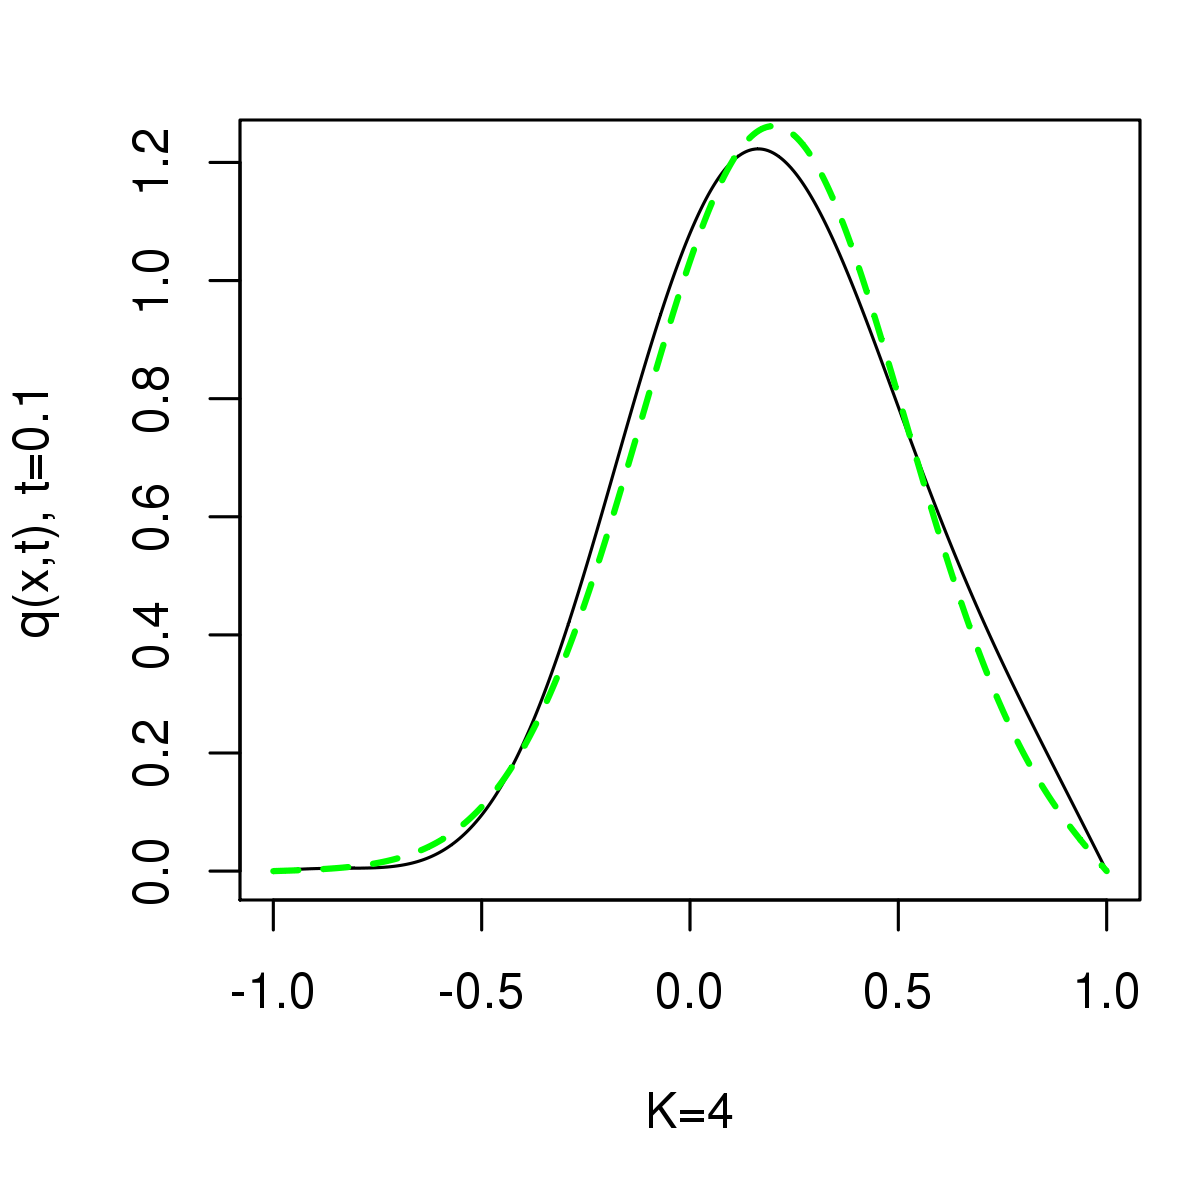
\includegraphics[width=1\linewidth]{{../R/finite-element-method/solution-K-4}.png}
    \end{minipage}
    & \begin{minipage}{0.25\textwidth}
      \centering
      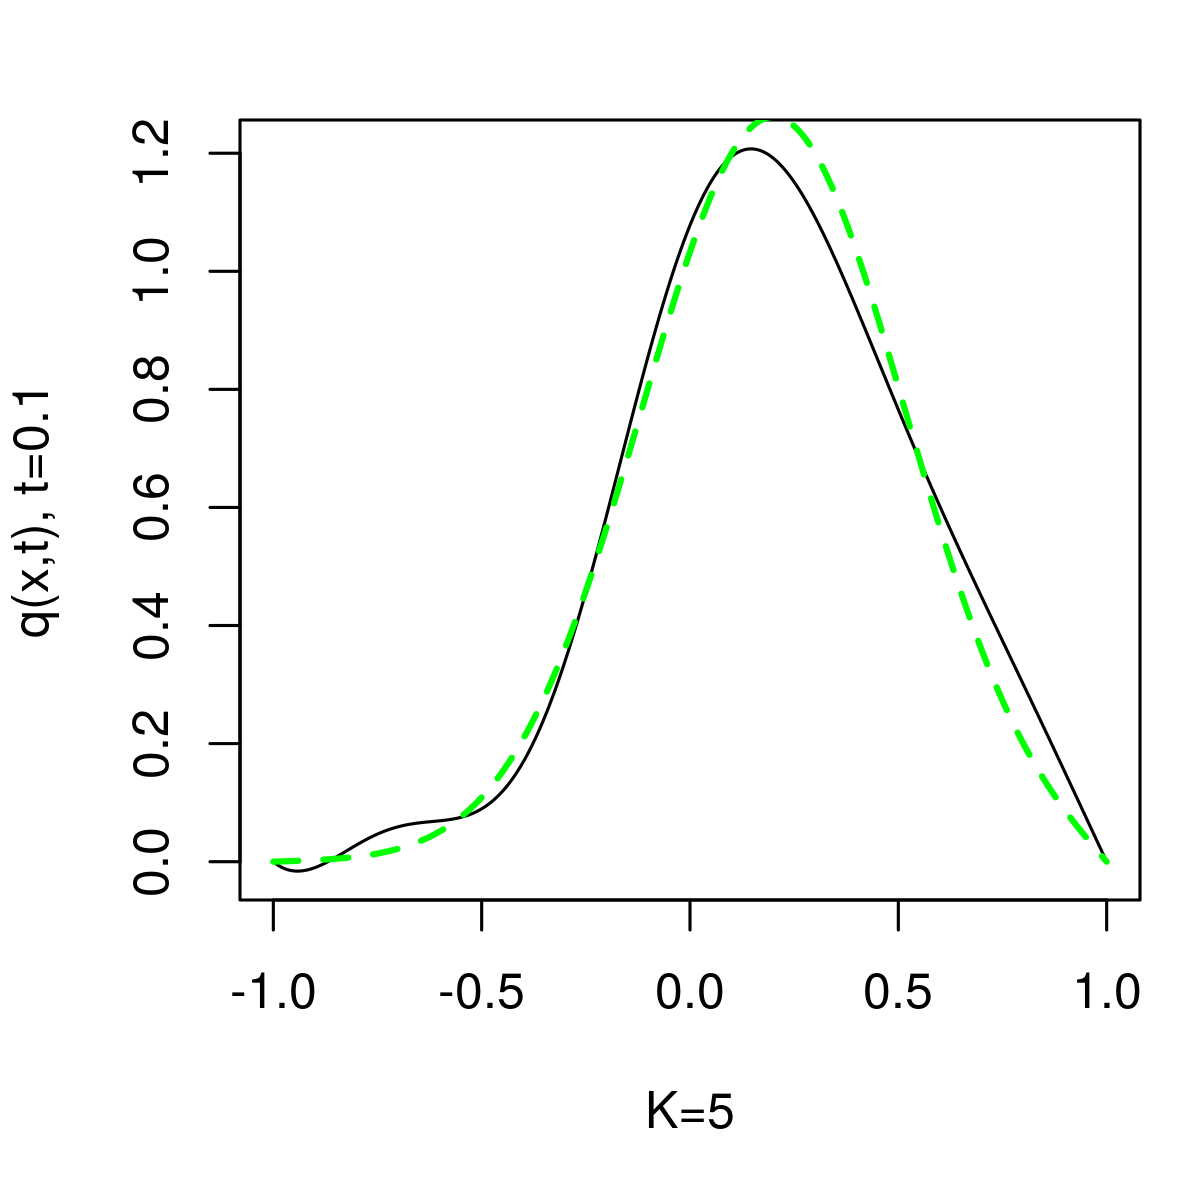
\includegraphics[width=1\linewidth]{{../R/finite-element-method/solution-K-5}.png}
    \end{minipage}
    & \begin{minipage}{0.25\textwidth}
      \centering
      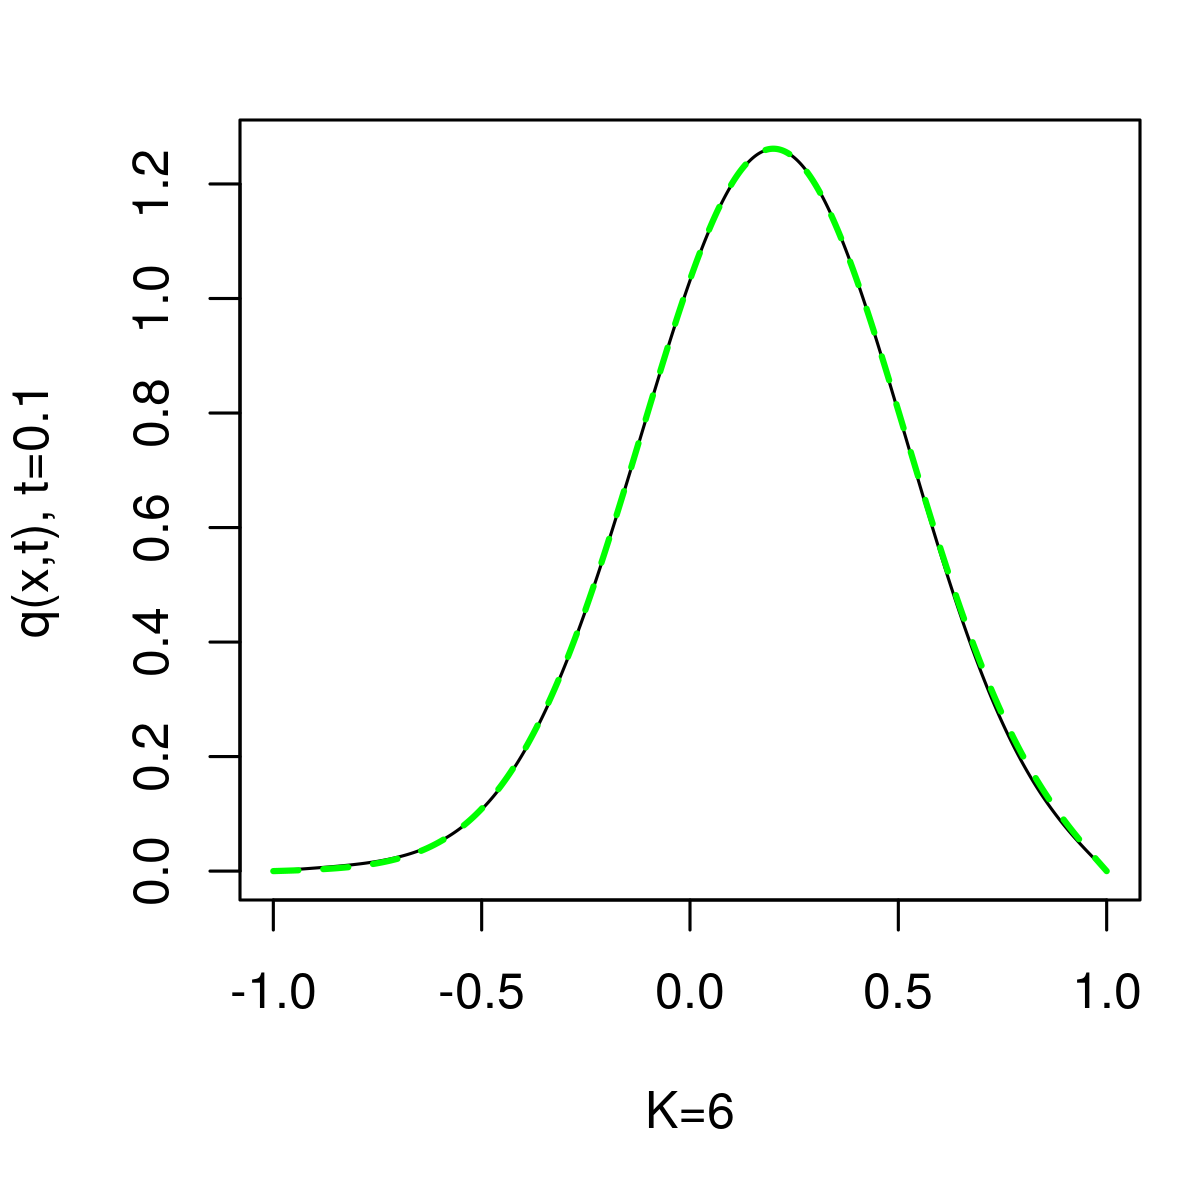
\includegraphics[width=1\linewidth]{{../R/finite-element-method/solution-K-6}.png}
    \end{minipage} \\
    \begin{minipage}{0.25\textwidth}
      \centering
      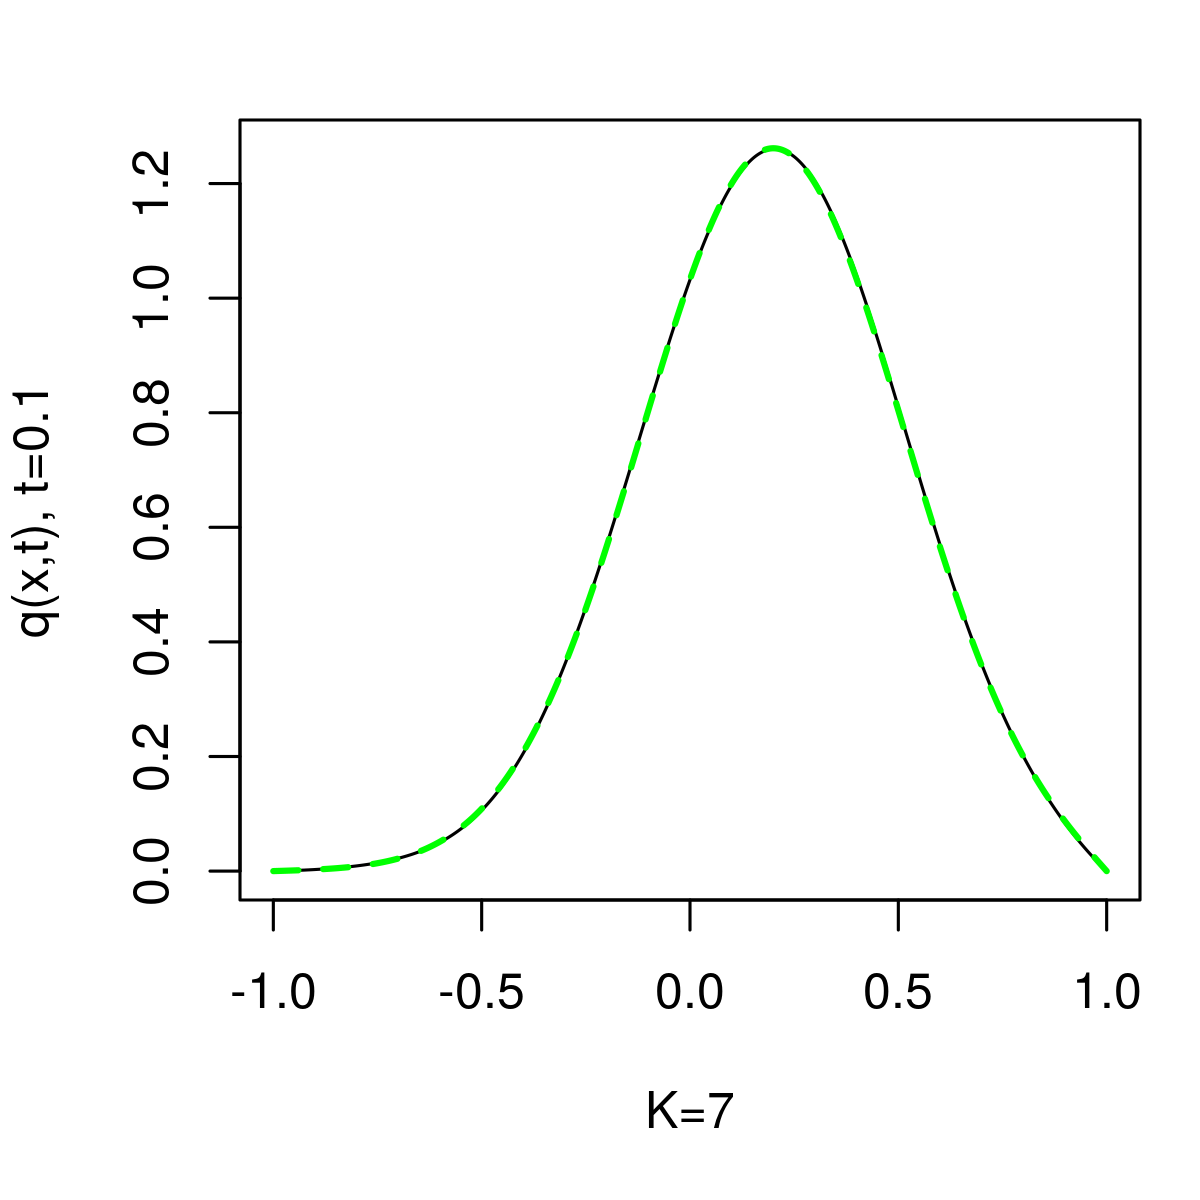
\includegraphics[width=1\linewidth]{{../R/finite-element-method/solution-K-7}.png}
    \end{minipage}
    & \begin{minipage}{0.25\textwidth}
      \centering
      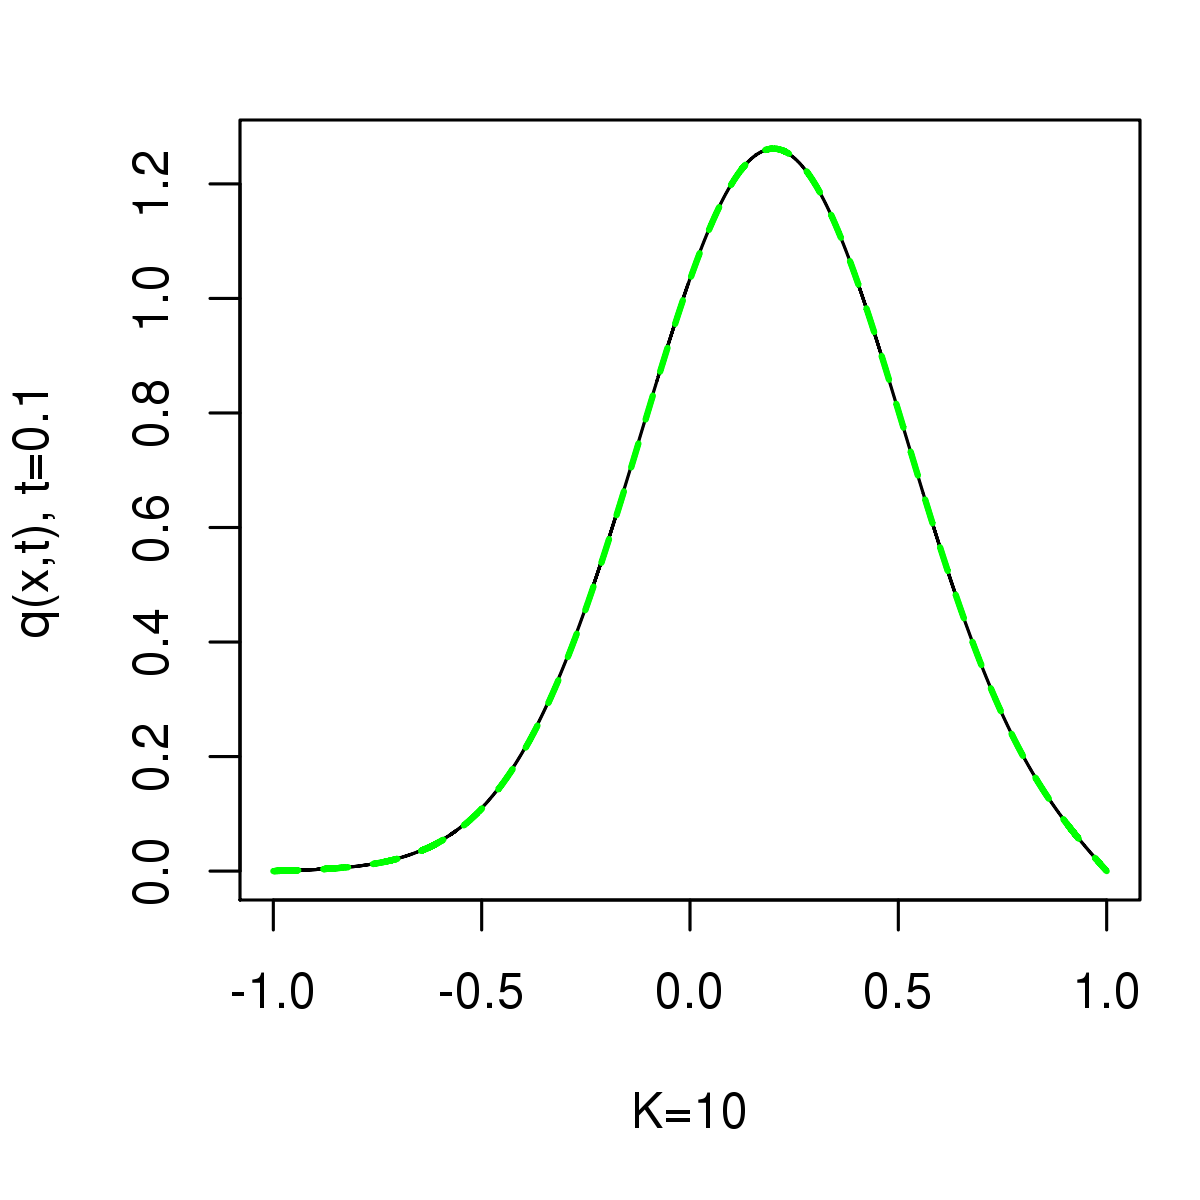
\includegraphics[width=1\linewidth]{{../R/finite-element-method/solution-K-10}.png}
    \end{minipage}
    & \begin{minipage}{0.25\textwidth}
      \centering
      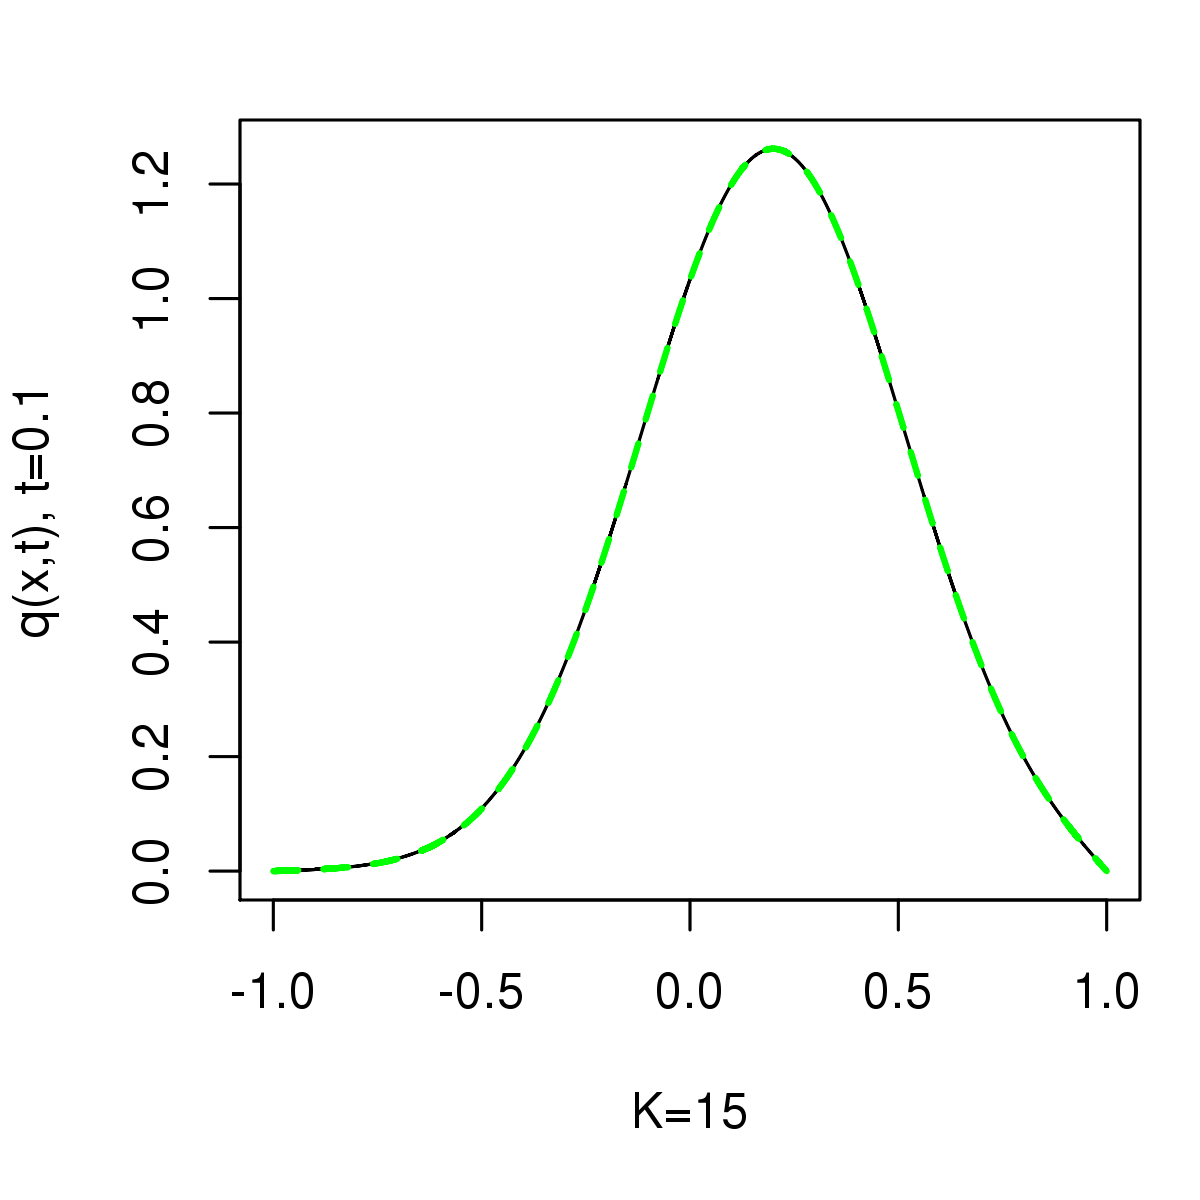
\includegraphics[width=1\linewidth]{{../R/finite-element-method/solution-K-15}.png}
    \end{minipage} \\
    \begin{minipage}{0.25\textwidth}
      \centering
    \end{minipage}
    & \begin{minipage}{0.25\textwidth}
      \centering
      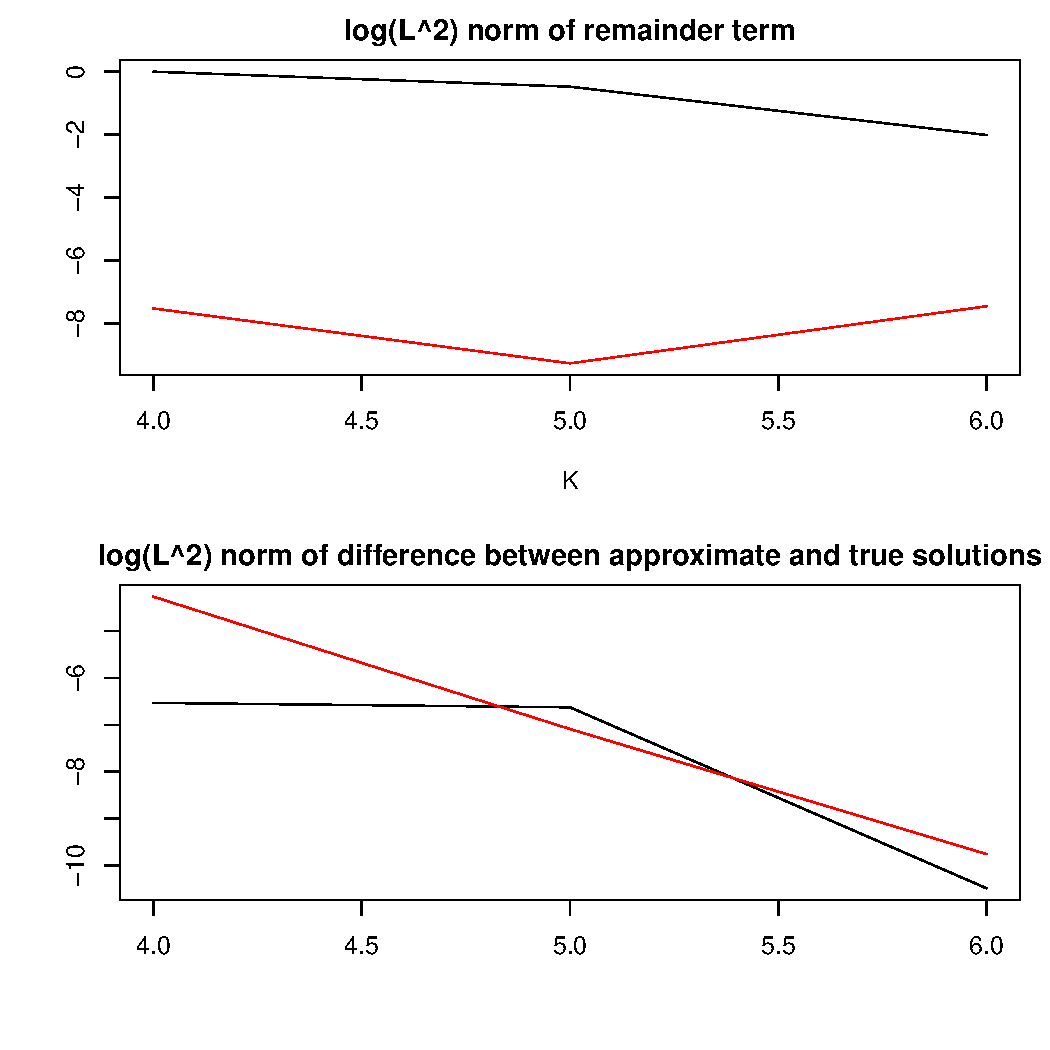
\includegraphics[width=1\linewidth]{{../R/finite-element-method/optimization-results}.pdf}
    \end{minipage}
    & \begin{minipage}{0.25\textwidth}
      \centering
    \end{minipage}
  \end{tabular}
  \caption{Approximate solution (solid black) and true solution
    (dashed green) for different number $K$ of optimally chosen basis
    elements
    $\left\{ (a-x)(b-x)\phi(x|\mu_k, \sigma_k^2) \right\}_{k=1}^K$.}
  \label{fig:optimized-sols}
\end{figure}

\subsection{Path-Integral Formulation and Differentiation With Respect
  to Boundaries}
The Taylor expansion of the semigroup operator in (\ref{eq:solution})
can be used to obtain the path-integral form for this problem:
\begin{align}
  \xi(t+\Delta t) &= e^{-\frac{1}{2}\sigma^2\, A\Delta t}\xi(t) \approx \left(I - \frac{1}{2}\sigma^2\, A \Delta t \right) \xi(t), \nonumber \\
  \Rightarrow q(x,t+\Delta t) &\approx \psi^T(x) \left(I - \frac{1}{2}\sigma^2\, A \Delta t \right) \xi(t), \label{eq:plus-dt}
\end{align}
for a small enought $\Delta t$. We will lend (\ref{eq:plus-dt}) a
\textit{probabilistic} interpretation. First, if we recall that the
elements in $\psi(x)$ are orthonormal, we will notice that the matrix
\[
  \displaystyle \int_\Omega \psi(x)\psi^T(x) dx = I.
\]
Therefore, we can re-write (\ref{eq:plus-dt}) as
\begin{align*}
  q(x,t+\Delta t) &\approx \psi^T(x) \left(I - \frac{1}{2}\sigma^2\, A \Delta t \right) \xi(t), \\
                  &= \psi^T(x) \left(I - \frac{1}{2}\sigma^2\, A \Delta t \right) e^{-\frac{1}{2}\sigma^2\, A t} \xi(0), \\
                  &= \displaystyle \int_\Omega \psi^T(x)
                    \left(I - \frac{1}{2}\sigma^2\, A \Delta t \right) \psi(y) \psi^T(y)
                    e^{-\frac{1}{2}\sigma^2\, A t} \xi(0) dy, \\
\end{align*}
The first and second parts in the integral are the probabilities
\begin{align*}
  P(X_{t+\Delta t} &= x, a < X_t < b, \forall t \in [t,t+\Delta t] |
                     X_t = y) \approx \psi^T(x) \left(I - \frac{1}{2}\sigma^2\, A \Delta
                     t \right) \psi(y) \\
  P(X_t &= y, a < X_t < b, \forall t \in [0,t] | X_0 = x_0) = \psi^T(y) e^{-\frac{1}{2}\sigma^2\, A t} \xi(0) \\
  \Rightarrow \displaystyle \int_\Omega P(X_{t+\Delta t} &= x, a < X_t < b, \forall t \in [t,t+\Delta t] |
                                                           X_t = y) P(X_t = y, a < X_t < b,
                                                           \forall t \in [0,t] | X_0 = x_0) dy \\
                   &\approx \displaystyle \int_\Omega \psi^T(x)
                    \left(I - \frac{1}{2}\sigma^2\, A \Delta t \right) \psi(y) \psi^T(y)
                    e^{-\frac{1}{2}\sigma^2\, A t} \xi(0) dy
\end{align*}
In general, again for small enough $\Delta t$,
\begin{align}
  P(X_t &= x, a < X_t < b, \forall t \in [0,t] | X_0 = x_0)
          \approx q_K(x,t) \approx \nonumber \\
        &\approx \int_\Omega \cdots \int_\Omega
          \left[ \psi^T(x)\left(I - \frac{1}{2}\sigma^2 A\Delta t\right)
          \psi(x_n) \right]
          \left[ \psi^T(x_{n-1})\left(I - \frac{1}{2}\sigma^2 A\Delta t\right)
          \psi(x_{n-2})\right] \cdots
          \left[ \psi^T(x_{1})\left(I - \frac{1}{2}\sigma^2 A\Delta t\right)
          \psi(x_{0})\right] dx_{n}\cdots dx_1 \label{eq:path-integral}
\end{align}
Equation (\ref{eq:path-integral}) is the \textbf{path integral
  formulation} for the solution to the initial-BV problem. We can
reduce (\ref{eq:path-integral}) to
\[
  q_K(x,t) \approx \psi^T(x) \left(I - \frac{1}{2}\sigma^2A\Delta t
  \right)^{t/\Delta t} \psi(x_0).
\]

Before we take derivatives with respect to the boundaries, first note
\[
  P(X_t = x, a < X_t < b, \forall t \in [0,t] | X_0 = x_0) = P(X_t=x,
  \max_{t'\in [0,t]} \left\{ X_{t'} \right\} < b, \min_{t'\in [0,t]}
  \left\{ X_{t'} \right\} > a | X_0 = x_0) = q(x,t).
\]
Hence,
\begin{equation}
  P\left(X_t = x, \max_{t'\in [0,t]} \left\{ X_{t'} \right\} = b, \min_{t'\in [0,t]}
  \left\{ X_{t'} \right\} = a | X_0 = x_0\right) =
  -\frac{\partial^2}{\partial a \partial b} q(x,t).
\end{equation}
This is what we are after. To compute the derivative, we can do
\begin{equation}
  -\frac{\partial^2}{\partial a \partial b} q(x,t) \approx
  -\frac{\partial^2}{\partial a \partial b} \left( \psi(x)^T \left( e^{-\frac{1}{2}\sigma^2\, At} \right) \psi(0) \right) \approx
  -\frac{\partial^2}{\partial a \partial b}
  \left(\psi^T(x) \left(I - \frac{1}{2}\sigma^2A\Delta t
    \right)^{t/\Delta t} \psi(x_0) \right).
\end{equation}
The above derivatives are expensive to compute. Moreover, at a first
glance, they have no immediate probabilistic interpretation. However,
under the path-integral formulation, they do. From
(\ref{eq:path-integral})
\begin{align}
  -\frac{\partial^2}{\partial a \partial b} q_K(x,t) = \int_\Omega \cdots \int_\Omega
  -\frac{\partial^2}{\partial a \partial b} \left(
  \left[ \psi^T(x)\left(I - \frac{1}{2}\sigma^2 A\Delta t\right)
  \psi(x_n) \right]
  \cdots
  \left[ \psi^T(x_{1})\left(I - \frac{1}{2}\sigma^2 A\Delta t\right)
  \psi(x_{0})\right] \right) dx_{n}\cdots dx_1.
\end{align}
Note that I have placed the derivatives on the inside of the
integral. This follows from the Dominated Convergence Theorem since
the derivatives are bounded over $\Omega$. This is not cheaper than
the other representations, however, consider one of the elements in
the sum of derivatives:
\[
  -\int_\Omega \cdots \int_\Omega \frac{\partial}{\partial a} \left[
    \psi^T(x)\left(I - \frac{1}{2}\sigma^2 A\Delta t\right) \psi(x_n)
  \right] \cdots \frac{\partial}{\partial b}\left[
    \psi^T(x_{1})\left(I - \frac{1}{2}\sigma^2 A\Delta t\right)
    \psi(x_{0})\right] dx_{n}\cdots dx_1.
\]
The above expression is the probability
\[
  P(X_t = x, \min\left\{ X_t \right\} = a, \max\left\{ X_t \right\} =
  b, \tau_a \in [t_n, t], \tau_b \in [0,t_1] | X_0 = x_0), 
\]
where $\tau_a(\tau_b)$ is the time when $X_t$ reaches boundary
$a\,\, (b)$. This motives us to write down
\[
  q(x,t | \tau_a \in \Delta t_k, \tau_b \in \Delta t_l ) =
  -\int_\Omega \cdots \int_\Omega \frac{\partial}{\partial a} \left[
    \psi^T(x)\left(I - \frac{1}{2}\sigma^2 A\Delta t\right) \psi(x_n)
  \right] \cdots \frac{\partial}{\partial b}\left[
    \psi^T(x_{1})\left(I - \frac{1}{2}\sigma^2 A\Delta t\right)
    \psi(x_{0})\right] dx_{n}\cdots dx_1.
\]
Therefore, in the context of MCMC, if we introduce the auxiliary
variables $\tau_a, \tau_b$, we can make evaluations of the likelihood
much faster. The next questions is, therefore, how to sample the
hitting times $\tau_a$ and $\tau_b$.

\subsection{Sampling hitting times}
Let $\tau$ be the first hitting time for $\Omega$. By definition of our solution $q(x,t)$,
\begin{align*}
  P(\tau > t) &= \int_\Omega q(x,t) dx \Rightarrow P(\tau \leq t) = 1 - \int_\Omega q(x,t) dx \\
  p(\tau = t) &= -\frac{\partial}{\partial t}\int_\Omega q(x,t) dx
\end{align*}

\bibliographystyle{plainnat}
% \bibliographystyle{bka}
\bibliography{master-bibliography}
\end{document}
